\chapter{Introdução}
A Diabetes Melito é uma doença que surge quando o organismo deixa de produzir insulina ou quando essa passa a não atuar com a mesma eficácia. Atualmente existe duas classificações para ela: Diabetes Melito tipo 1 e 2. A primeira se caracteriza por ser autoimune que lesa, de forma irreversível, as células do pâncreas, produtoras de insulina e conhecidas como células beta, e seu diagnóstico se dá durante a infância do portador. Enquanto a segunda é consequência da resistência do próprio organismo contra as ações da insulina, o principal fator para se desenvolver essa resistência é a obesidade\cite{portaldiabetes2008}.
Bomba de infusão de insulina é um pequeno aparelho eletrônico, do tamanho de um celular ou pager, que está ligado ao corpo do portador da doença por um finíssimo cateter com uma agulha flexível na ponta. Essa agulha é inserida no braço, coxa ou abdômen e deve ser trocada em um período de 2 ou 3 dias. Essa bomba não mede o índice glicêmico ou a quantidade de insulina a ser utilizada, essa medição é feita através do glicosímetro. A Figura ~\ref{fig:bombainfusao}\footnote{\url{http://www.diabetes.org.br/sala-de-noticias/2316-bombas-de-infusao-de-insulina}} representa um aparelho comercial.

\begin{figure}[htp]
	\centering
	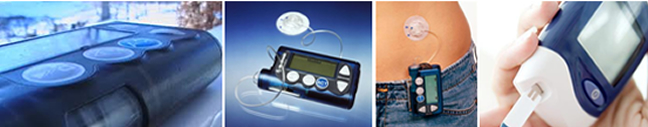
\includegraphics[scale=1]{images/bombainsulina.png}
	\caption{Imagens de uma bomba de infusão de insulina}	
	\label{fig:bombainfusao}	
\end{figure}


Seu funcionamento é bem simples, libera-se uma quantidade de insulina, programada pelo médico, durante o dia todo, simulando o funcionamento do pâncreas de uma pessoa saudável, entretanto existem cuidados a serem tomados: calcular a quantidade de carboidratos ingeridos a cada refeição e programar o aparelho para injetar uma quantidade de insulina com maior velocidade no organismo nos horário em que se faz as refeições principais.
Quanto a quem pode usar, a pessoa deve cumprir alguns pré-requisitos que são:
\begin{itemize}
\item Conseguir medir o índice glicêmico no mínimo 4 vezes por dia;
\item Durante a fase de adaptação e ajuste da dosagem a serem utilizadas pela bomba, fazer a medição glicêmica de 6 a 8 vezes por dia;
\item Seguir as recomendações médicas além de manter contato e um constante \emph{feedback} com os responsáveis pela bomba e, além de tudo, seguir a dieta recomendada, respeitando quantidades ingeridas;
\item Ter condição financeira para custear o equipamento e o contato com os responsáveis por ele;
\item Estar disposto ao uso da bomba durante o dia todo, 24 horas junto ao corpo;
\item Aprender sobre contagem de carboidratos para saber seu consumo durante as refeições;
\item Praticar exercícios.
\end{itemize}

Cumprindo os pré-requisitos citados temos as vantagens de seu uso que são:

\begin{itemize}
\item Maior flexibilidade no horário das refeições;
\item Se usada corretamente o risco de hipoglicemia é reduzido, e a longo prazo as complicações devido ao diabetes também;
\item Melhora o controle glicêmico;
\item Melhora no controle do fenômeno do amanhecer, responsável pelo aumento do índice glicêmico durante a manha, entre as 4 e 8 horas da manha, causador da hipoglicemia se o diabético não calculou a dose de insulina antes de dormir, ou não se levantou durante a noite para gerenciá-la.
\end{itemize}

Mas mesmo com todas as vantagens dada devido ao uso do equipamento caso o diabético seja obeso, ingira grandes quantidades de alimento ou açúcar, ou seja, carboidratos, não praticar atividades físicas, não fazer a medição do índice glicêmico na quantidade de vezes recomendada, ou até mesmo determinar por si só a quantidade de insulina a ser utilizada, não existe vantagem no seu uso.
É importante ter em mente que mesmo com toda facilidade e tecnologia existente o acompanhamento médico não deve ser deixado de lado. As principais indicações médicas para o uso do equipamento são:

\begin{itemize}
\item Fenômeno do amanhecer;
\item Hipoglicemia;
\item Diminuir a variação do índice glicêmico;
\item Hiperglicemia;
\item Recorrente ceatosidade, que é o acumulo de ceatócidos, pois o fígado quebra a gordura e proteína devido à falta de insulina, pois o corpo não consegue utilizar a glicose como energia;
\item Flexibilidade, especialmente para crianças pequenas;
\item Gestação, viagens e atividade físicas;
\item Fobia de injeção;
\item Desejo do diabético \cite{diabetes2013, portaldiabetes2009}.
\end{itemize}

\section{Motivação}
Segundo a Sociedade Brasileira de Diabetes \cite{sbc2014}, diversos estudos realizados mostram que o tratamento feito através da Infusão de insulina tem diversas melhorias quando comparado com outros tratamentos existentes. Entretanto não é o mais utilizado devido ao seu alto custo, devido a importação.
Logo, esse projeto vem com foco social: facilitar o acesso da população brasileira de baixa renda ao equipamento, melhorando sua qualidade de vida dos portadores da doença que se encaixem nesse perfil. 

\section{OBJETIVOS}
Esse projeto tem como objetivo principal desenvolver um software para um protótipo de uma Bomba de Infusão de insulina utilizando o microcontrolador da família PIC, PIC18F452. 

\subsection{OBJETIVOS SECUNDÁRIOS}

Em segundo plano este trabalho foca em:
\begin{itemize}
\item Aprendizado sobre as características e funcionalidades disponíveis do microcontrolador escolhido;
\item Aprendizado das tecnologias utilizadas como: compilador, simulador e bibliotecas disponíveis;
\item Desenvolvimento das funcionalidades básicas de uma bomba de infusão de insulina;
\item Aprendizado sobre a escolha e uso de um motor de passo;
\item Aprendizado sobre a forma de uso de um \emph{display} de LCD para comunicação com o usuário.
\end{itemize}

\section{PROCEDIMENTOS METODOLÓGICOS}
Este trabalho foi dividido em duas etapas: pesquisa para levantamento de referências bibliográficas e desenvolvimento prático. Durante a primeira etapa, foi feita a pesquisa e levantamento bibliográfico sobre o tema em questão para que fosse possível um melhor entendimento da plataforma, tecnologias e, claro, do problema abordado. Juntamente com essa pesquisa, foi feito um estudo sobre o microcontrolador PIC escolhido, PIC18F452, a partir do material encontrado. O estudo e desenvolvimento foi feito utilizando o compilador MikroC e sua IDE, já para os testes utilizou-se o simulador Proteus. Em seguida houve-se um levantamento de informações sobre sistemas embarcados, sistemas críticos e sistemas críticos de tempo real, e assim adquirindo-se conhecimento sobre os conceitos de desenvolvimento da área em questão, uma vez que a confiabilidade e segurança do problema proposto é importantíssimo.


O software de controle do protótipo da bomba de infusão de insulina foi desenvolvido na linguagem C, compilado para o microcontrolador já citado, PIC18F452. O sistema é responsável basicamente por gerenciar o perfil de infusão basal, calcular intervalos corretos e passos necessários para uma infusão. Desta forma, o
software foi dividido nos seguintes módulos: Config, LCD, InsulinPump, Motor, Menu, TimerMotor e principal. 

Essa divisão por módulos é, e foi, extremamente importante para o desenvolvimento do sistema. Somando-a à um dos conceitos mais importante desse projeto - OOC, \emph{Object-Oriented Programming With ANSI-C} - são as chaves para a facilidade de manutenção, entendimento do código e possível evolução do projeto.

As responsabilidade dos módulos são bem claras e isoladas:

Config: Centralizar configurações gerais do sistema;
LCD: Abstrair uso do periférico para o resto do sistema;
InsulimPump: Abstrair funcionamento, requisitos de segurança e outras particularidades da bomba;
Motor: Abstrai como se controla o motor e qual tipo está sendo utilizado para infusão;
TimerMotor: Separa o gerenciador de tempo das particularidade únicas do hardware e compilador;
Menu: Facilitar navegação entre menus, simulando máquina de estado;
Principal: Possui o \emph{loop} principal para navegação simples entre os menus existentes.

Os testes do software foram feitos através do simulador Proteus, desenvolvido pela Labcenter. Ferramenta tão importante quanto o OOC para o caminhar deste trabalho. Permite um alto nível de testes, devido a sua facilidade de uso, além do grande auxílio à depuração. O uso do simulador durante o desenvolvimento do software acarreta na minimização dos problemas de integração entre hardware e software, complicações estas que são praticamente impossíveis de estimar. 

E, finalizando, após o desenvolvimento, executou-se uma bateria de testes para se o funcionamento da bomba estava sendo de acordo coma forma especificada, levando em conta toda a integração necessária com os periféricos existentes.
